\section{Yêu cầu và tiêu chí đánh giá}\label{sec:01-foundations-requirements}
\subsection{Vai trò người dùng và luồng nghiệp vụ}
Người gửi tạo SOS hoặc báo cáo có mô tả/ảnh, cung cấp vị trí khi có thể và nhận phản hồi trạng thái. Điều phối viên xem bản đồ, danh sách và hàng xem xét; xác minh thông tin, giao đội và ghi nhận kết quả. Nhóm nghiên cứu chuẩn bị dữ liệu, cấu hình và phân tích artifact mà không đưa nhãn đánh giá vào luồng suy luận.

Một luồng nghiệp vụ tối thiểu bắt đầu bằng tạo báo cáo tại thiết bị, ghi vào lưu trữ cục bộ, chọn chế độ gửi, nhận ACK, đưa báo cáo vào danh sách xử lý và cập nhật phản hồi. Khi mất mạng, báo cáo cần giữ được định danh và payload để tiếp tục ở lần gửi sau. Nếu thiếu GPS, báo cáo được chuyển vào hàng xem xét; gán một tọa độ mặc định sẽ tạo một điểm đến sai có vẻ hợp lệ.

\begin{figure}[htbp]
\centering
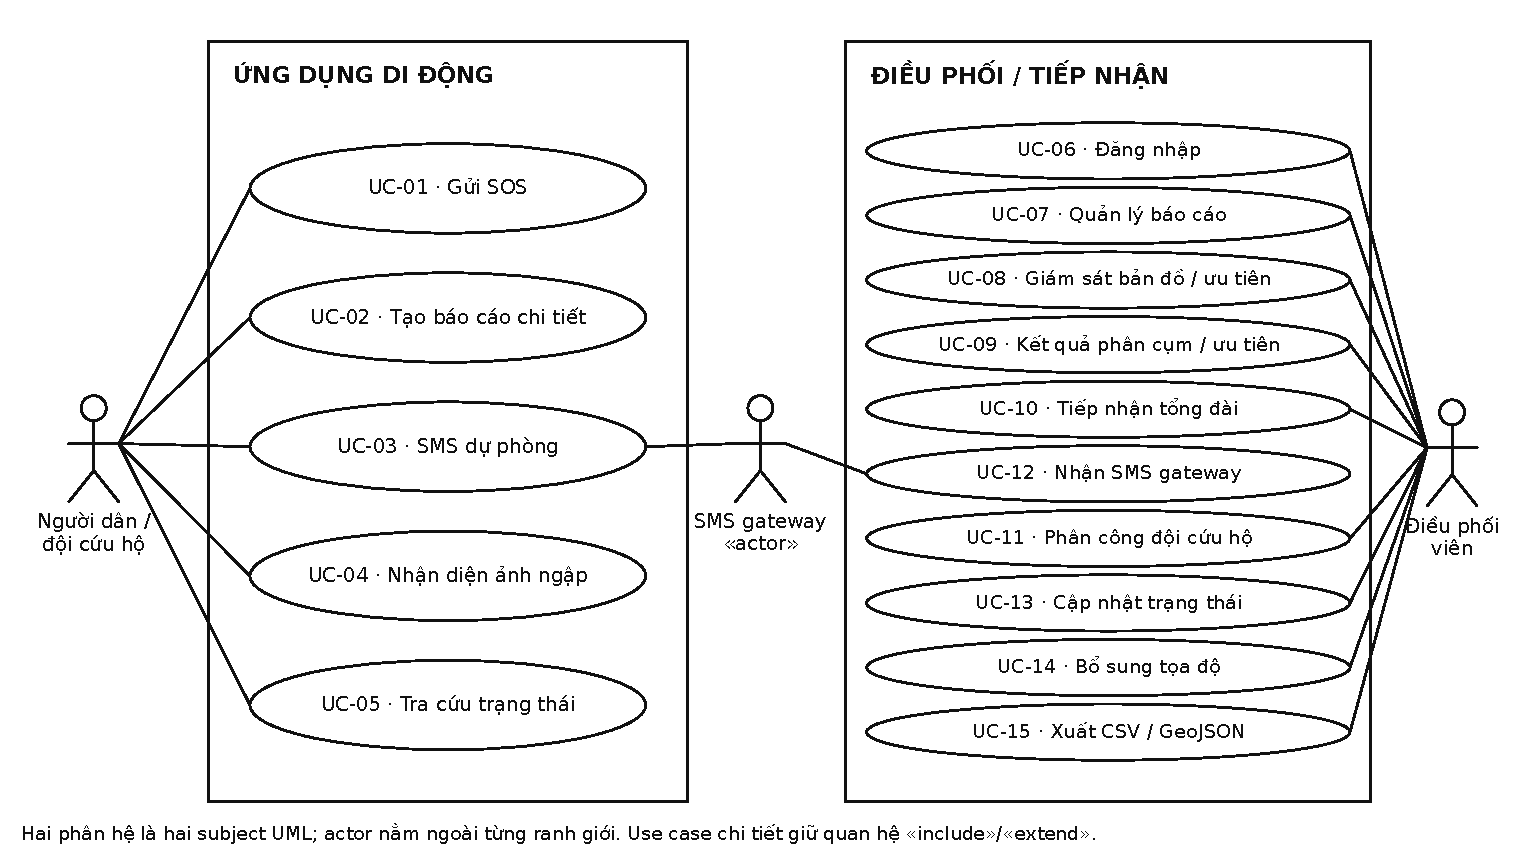
\includegraphics[width=\textwidth]{usecase.pdf}
\caption{Sơ đồ Use Case tổng thể toàn hệ thống cứu hộ}
\label{fig:usecase-overall}
\end{figure}

\begin{figure}[htbp]
\centering
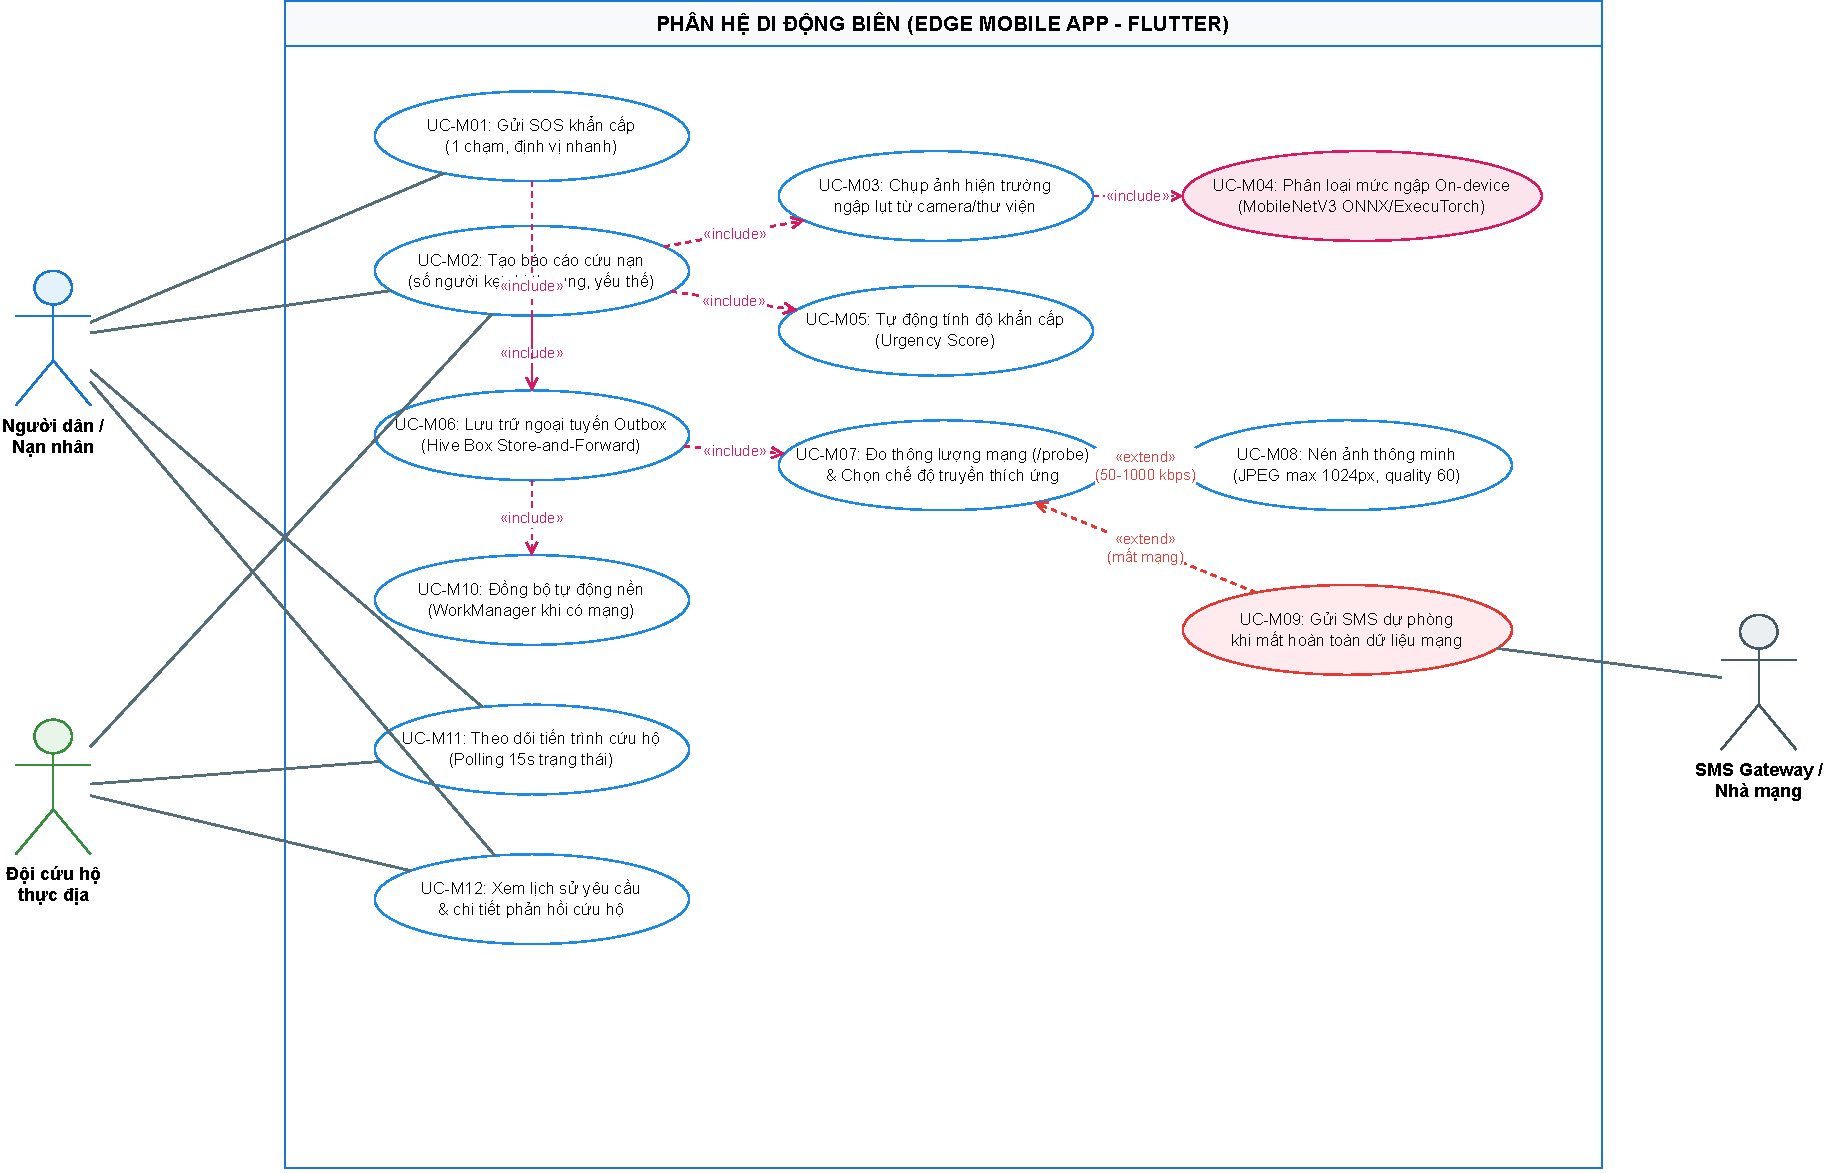
\includegraphics[width=\textwidth]{usecase_mobile.pdf}
\caption{Sơ đồ Use Case phân hệ ứng dụng di động phía người dân và đội cứu hộ}
\label{fig:usecase-mobile}
\end{figure}

\begin{figure}[htbp]
\centering
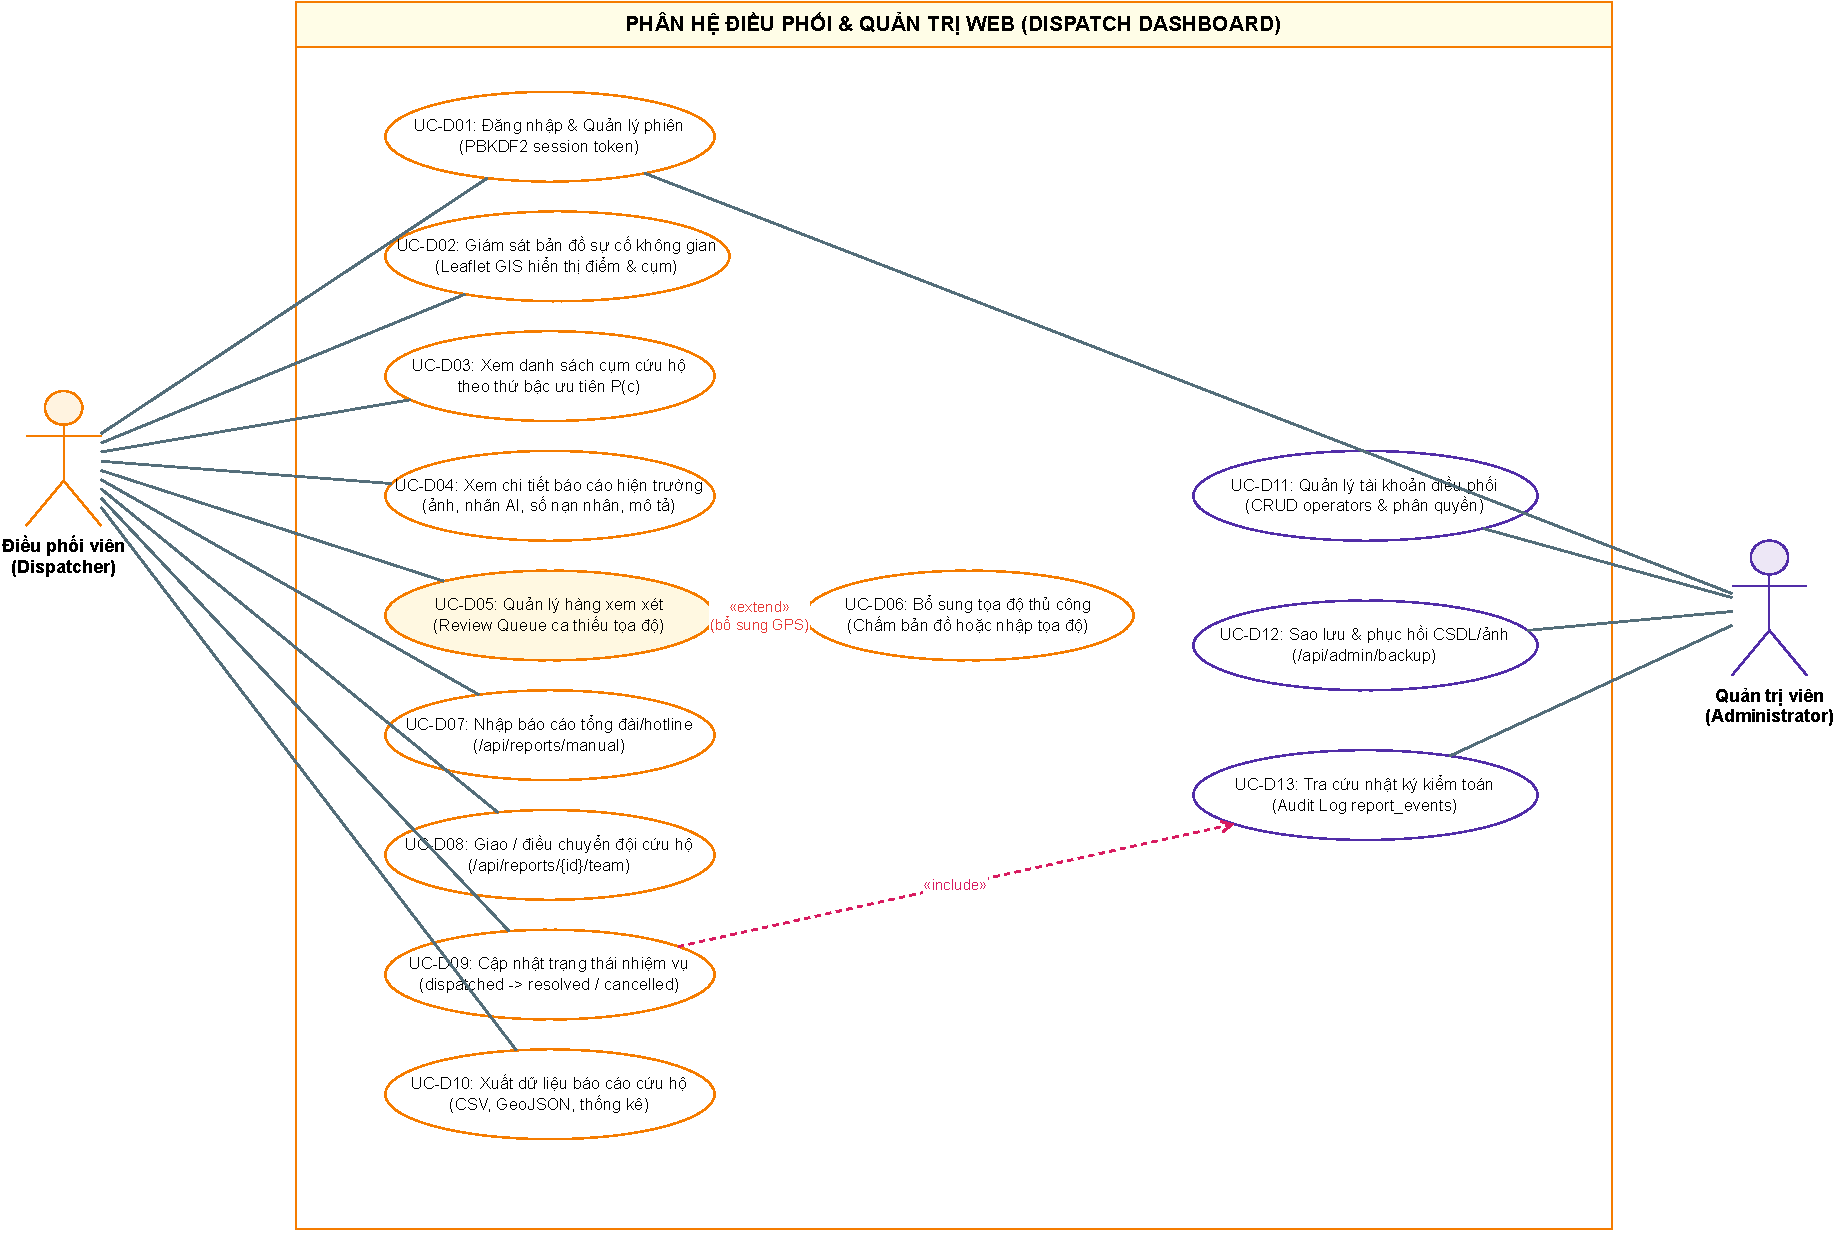
\includegraphics[width=\textwidth]{usecase_dashboard.pdf}
\caption{Sơ đồ Use Case phân hệ Web Dashboard phục vụ điều phối tác chiến}
\label{fig:usecase-dashboard}
\end{figure}

\subsection{Yêu cầu chức năng}
\begin{longtable}{P{.10\textwidth}P{.40\textwidth}P{.39\textwidth}}
\caption{Yêu cầu chức năng và căn cứ kiểm chứng}\label{tab:functional-requirements}\\
\toprule Mã & Yêu cầu & Căn cứ kiểm chứng \\\midrule\endfirsthead
\toprule Mã & Yêu cầu & Căn cứ kiểm chứng \\\midrule\endhead
F01 & Tạo SOS và bài báo cáo; cho phép thiếu ảnh hoặc GPS & Luồng tạo bản ghi, test tích hợp, hàng xem xét của API cụm \\
F02 & Lưu cục bộ trước khi gửi; gửi lại khi có mạng & Hive outbox, repository, test mất mạng/có mạng lại \\
F03 & Phân loại mức ngập từ ảnh trên thiết bị khi đủ asset/runtime & Mã suy luận native; đối chiếu runtime CPU; kiểm chứng điện thoại trình bày riêng \\
F04 & Chọn ảnh gốc, ảnh nén hoặc metadata theo mạng/confidence & Hàm chọn chế độ thuần và test chính sách gửi \\
F05 & Chống gửi lặp, kiểm tra xung đột định danh & Hợp đồng message, hash JCS, test ACK/hash/sequence \\
F06 & Gom cụm và xếp hạng từ trường quan sát & Lõi thuật toán, adapter và benchmark RQ1/RQ2 \\
F07 & Điều phối và cập nhật trạng thái có nhật ký & API dashboard, bảng sự kiện, test chuyển trạng thái \\
F08 & Xem bản đồ, lọc báo cáo, xuất dữ liệu & Dashboard Leaflet, API truy vấn và CSV/GeoJSON \\
F09 & Tiếp nhận từ SMS gateway và nhập tổng đài & Endpoint có xác thực gateway và luồng nhập thủ công; vận hành viễn thông cần kiểm chứng riêng \\
\bottomrule
\end{longtable}

\subsection{Yêu cầu phi chức năng}
Tính toàn vẹn dữ liệu yêu cầu payload có cấu trúc rõ, số hữu hạn trong miền hợp lệ và transaction theo message. Tính bền vững yêu cầu tách bộ nhớ giao diện khỏi lưu trữ cục bộ và đảm bảo gửi lại sau gián đoạn. Tính nhất quán yêu cầu trạng thái chỉ đi theo các chuyển hợp lệ và version tăng. Tính giải thích yêu cầu truy được nguồn số liệu, quy tắc ánh xạ, cấu hình và phạm vi kiểm thử.

Hiệu năng truyền tải và độ trễ suy luận là các chỉ tiêu kỹ thuật then chốt của hệ thống. Ứng dụng di động cần đáp ứng thời gian phản hồi nhanh trong khâu trích xuất đặc trưng ngập lụt, đồng thời giảm thiểu lưu lượng dữ liệu truyền qua mạng di động trong điều kiện nghẽn mạng. Việc tối ưu hóa mức tiêu thụ năng lượng và thử nghiệm trên diện rộng nhiều dòng thiết bị thực tế là định hướng tiếp tục hoàn thiện.

Phân quyền và bảo mật điều phối được đảm bảo thông qua cơ chế quản lý tài khoản, mã hóa mật khẩu, kiểm soát phiên làm việc dựa trên mã token và phân định rõ ràng giữa vai trò quản trị viên (Admin) và điều phối viên tác chiến (Operator). Các thao tác can thiệp dữ liệu, phân công đội cứu hộ và cập nhật trạng thái đều được lưu vết phục vụ công tác giám sát.

\subsection{Ma trận mục tiêu--thước đo}
\begin{longtable}{P{.29\textwidth}P{.28\textwidth}P{.32\textwidth}}
\caption{Thước đo theo tầng và phạm vi đánh giá}\label{tab:metric-map}\\
\toprule Tầng & Chỉ số/kiểm tra & Phạm vi đánh giá \\\midrule\endfirsthead
\toprule Tầng & Chỉ số/kiểm tra & Phạm vi đánh giá \\\midrule\endhead
Ảnh & Accuracy, macro-F1, recall lớp, ma trận nhầm lẫn & Phân loại trên tập kiểm tra chuẩn hóa \\
Tối ưu mô hình & Kích thước, độ suy giảm chất lượng, độ trễ, đồng thuận top-1 & Đánh đổi tài nguyên và độ chính xác giữa các định dạng \\
Khẩn cấp có cấu trúc & Độ khớp quy tắc trên các tổ hợp trạng thái & Khả năng trích xuất điểm khẩn cấp từ thuộc tính \\
Phân cụm & ARI, pairwise F1, tỷ lệ điểm đến giả & Chất lượng phân hoạch sự cố trong các kịch bản thực nghiệm \\
Xếp hạng & NDCG@5, Spearman, độ trôi thứ tự & Mức độ tương đồng với độ khẩn cấp thực và độ ổn định dưới nhiễu \\
Điều phối & Mức độ tổn thất mô phỏng, tỷ lệ trễ hạn & Hiệu quả phân bổ nguồn lực cứu nạn \\
Đồng bộ & Khử trùng, giải quyết xung đột, nhất quán phiên bản & Độ tin cậy truyền nhận trong điều kiện mạng gián đoạn \\
\bottomrule
\end{longtable}

\subsection{Nguyên tắc xử lý dữ liệu không hoàn chỉnh}
Trong điều kiện thực tế, thông tin cứu hộ thường xuyên gặp tình trạng thiếu dữ liệu. Hệ thống phân biệt rõ giữa trường hợp dữ liệu có giá trị bằng không (như mức ngập bằng 0) và trường hợp thiếu dữ liệu (người dùng không gửi ảnh hoặc không bật GPS). Các báo cáo thiếu vị trí địa lý được tự động chuyển vào hàng đợi xem xét riêng để điều phối viên bổ sung thủ công qua phỏng vấn hoặc nghiệp vụ ngoại tuyến, tuyệt đối không gán tọa độ giả định nhằm tránh điều động sai hiện trường.

Về mặt thời gian, hệ thống ưu tiên lưu giữ thời điểm ghi nhận ban đầu tại thiết bị biên (\texttt{createdAt}) song song với thời điểm tiếp nhận tại máy chủ (\texttt{receivedAt}). Cách tiếp cận này giúp phân biệt độ trễ truyền thông với thời gian phát sinh sự cố, đảm bảo tính khách quan khi thuật toán tái hiện trình tự diễn biến thiên tai.
